\documentclass[a4paper,10pt]{article}


\usepackage[utf8]{inputenc}
\usepackage{graphicx}
\usepackage{hyperref}
\usepackage{color}
\usepackage{listings}

\title{White-Rabbit Node-Core Software}
\author{Federico Vaga $<$federico.vaga@cern.ch$>$\\CERN - BE-CO-HT}
\date{December 2014}

\pdfinfo{%
  /Title    (White-Rabbit Node-Core Software)
  /Author   (Federico Vaga <federico.vaga@cern.ch>, CERN - BE-CO-HT)
  /Creator  (Federico Vaga <federico.vaga@cern.ch>, CERN - BE-CO-HT)
  /Producer ()
  /Subject  (White-Rabbit Node-Core Software Documentation)
  /Keywords (white rabbit node core documentation)
}

\begin{document}
\setlength{\parindent}{0cm}
\setlength{\parskip}{3mm}
\maketitle
\lstset{language=C, basicstyle=\footnotesize\bfseries, 
keywordstyle=\color{blue},}

\section{Introduction}
This is the manual of the driver and the library for the
\textit{White-Rabbit Node-Core} HDL core developed on the \textbf{Open
  HardWare Repository}\footnote{http://www.ohwr.org/projects/wr-node-core-sw}

The goal of this manual is to explain you how to retrieve, install
and using the software. This manual does not explain details about
the White-Rabbit Node-Core or its internal behavior. If you want to
know more about the White-Rabbit Node-Core, please refer to the HDL
documentation.

Here you will not find the API details. For API documentation,
generate the Doxygen documentation by running the following command:

\begin{verbatim}
  cd doc
  make doxygen
\end{verbatim}

The HTML documentation will be available in the directory
\texttt{doxy-wrnc}

%%%%%%%%%%%%%%%%%%%%%%%%%%%%%%%%%%%%%%%%%%%%%%%%%%%%%%%%%%%%%%%%%%%%%%
\section{Repository}%%%%%%%%%%%%%%%%%%%%%%%%%%%%%%%%%%%%%%%%%%%%%%%%%
This project is hosted on the Open HardWare Repository at the
following link \url{http://www.ohwr.org/projects/wr-node-core-sw}

You can get the git repository using the following command:
\begin{verbatim}
  git clone --recursive
     git://ohwr.org/white-rabbit/wr-node-core/wr-node-core-sw.git
\end{verbatim}

The repository is organized as following:
\begin{description}
  \item[kernel] this directory contains all the driver's source files
  \item[lib] this directory contains all the library source files
  \item[tools] this directory contains the sources for a set of simple
    tools.
  \item[applications] this directory contains a collection of
    applications where the White-Rabbit Node-Core is involved. Each
    application is documented separately
  \item[doc] this directory contains all the documentation of this
    project. Here, you can generate the doxygen documentation of the
    library and this manual as well.
\end{description}


\subsection{Dependencies}%%%%%%%%%%%%%%%%%%%%%%%%%%%%%%%%%%%%%%%%%%%%
All the software dependencies are part of the repository as git
sub-modules. The driver depends on the
\texttt{fmc-bus}\footnote{\url{http://www.ohwr.org/projects/fmc-bus}},
so you can find its git sub-module in the repository.

There is also a \texttt{svec-sw} sub-module. This is not a real
dependency but the SVEC is where probably you are going to use the
White-Rabbit Node-Core. This facilitate the package release and
distribution. It also allows us to give an indication about the
carrier compatibility.

Remember to use the \texttt{--recursive} option in order to clone also
all sub-modules

\begin{verbatim}
  git clone --recursive <repo-address>
\end{verbatim}

If you did not clone with the \texttt{--recursive} option, then update
the sub-modules with the following command

\begin{verbatim}
  git submodule update
\end{verbatim}


%%%%%%%%%%%%%%%%%%%%%%%%%%%%%%%%%%%%%%%%%%%%%%%%%%%%%%%%%%%%%%%%%%%%%%
\section{Installation}%%%%%%%%%%%%%%%%%%%%%%%%%%%%%%%%%%%%%%%%%%%%%%%
The driver depends on the \texttt{fmc-bus} driver, as well as the
Linux kernel. Also, it must talk to a specific FPGA binary with the
(White-Rabbit Node-Core inside) running in the carrier card. According
to the \texttt{fmc-bus} module, you have also to load the driver of
your carrier (\texttt{svec-sw} or \texttt{spec-sw})

The library does not have any dependency with other software packages.

\subsection{Gateware Installation}%%%%%%%%%%%%%%%%%%%%%%%%%%%%%%%%%%%
The White-Rabbit Node-Core is an HDL component; so, there is not
a dedicated gateware, but it can be part of any gateware. These
gatewares must be placed under \texttt{/lib/firmware} and loaded with
other fmc's drivers.
%FIXME it will change with UAL

\subsection{Software Installation}%%%%%%%%%%%%%%%%%%%%%%%%%%%%%%%%%%%
\subsubsection{Compilation}
There are not special requirements for the compilation, just run

\begin{verbatim}
  make
\end{verbatim}

Optionally, you can set the following environment variables to
customize you compilation:
\begin{description}
  \item[LINUX] path to a \textit{Linux} source directory
  \item[FMC\_BUS] path to a \textit{fmc-bus} directory
\end{description}

In order to compile for different environments, in the directories
\texttt{lib} and \texttt{tools} you can create a dedicated
\texttt{Makefile} to configure the environment before run the
project's \texttt{Makefile}. This dedicated \texttt{Makefile} must be
named \texttt{Makefile.specific}.

The compilation will produce the binary files in the respective
directories.

Note that the compilation process will also compile all the
applications under the directory \texttt{applications}.

\subsubsection{Library and Tools Installation}
Once you have compiled the library and tools you can install the
binaries in order to make them visible to the entire system.

\begin{verbatim}
  make install
\end{verbatim}

\subsubsection{Driver Loading}
You can place the driver wherever you want and load it using
\texttt{modporbe(8)} or \texttt{insmod(8)}.

The driver support the following module parameters:
\begin{description}
  \item[max\_slot\_msg] Maximum number of messages to keep in the
    driver internal queue for each slot.
\end{description}


%%%%%%%%%%%%%%%%%%%%%%%%%%%%%%%%%%%%%%%%%%%%%%%%%%%%%%%%%%%%%%%%%%%%%
\section{Software Usage}%%%%%%%%%%%%%%%%%%%%%%%%%%%%%%%%%%%%%%%%%%%%%
In figure~\ref{fig:swgenstack} you can see an overview of the software
stack and the White-Rabbit Node-Core internal components seen by the
driver.

\begin{figure}[ht]
	\centering
	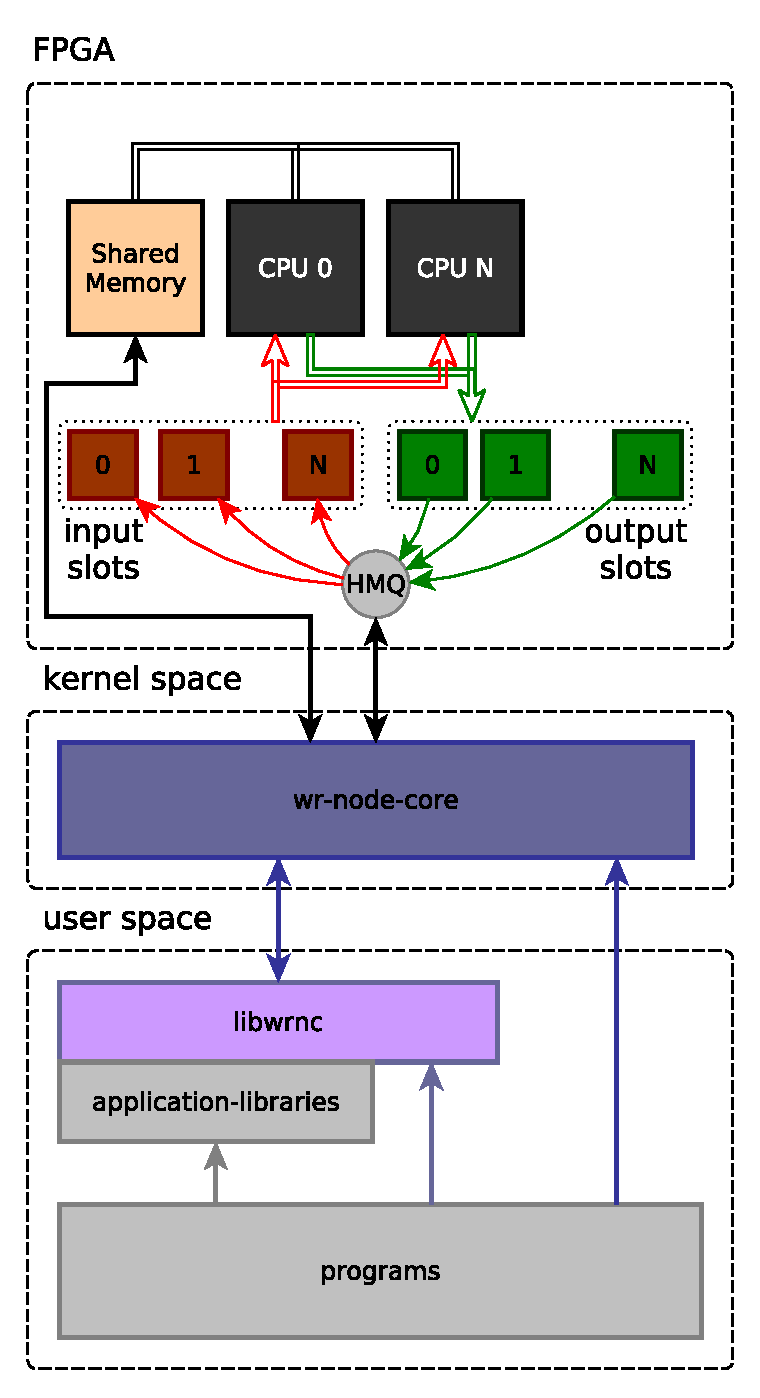
\includegraphics[scale=0.5]{img/sw-gen-stack.eps}
	\caption{White-Rabbit Node-Core Software Stack}
        \label{fig:swgenstack}
\end{figure}

Looking from the bottom to the top. The final user-space program has
three way to access the White-Rabbit Node-Core resources:

\begin{itemize}
  \item the application specific library. It is suggested to use these
    libraries for application-specific programs. Note that this kind of
    libraries may hide White-Rabbit Node-Core details/architecture.
  \item the White-Rabbit Node-Core library \texttt{libwrnc}. It can be
    used at any time when the specific library does not provide all
    functionality.
  \item the driver's sysfs attributes and char devices
\end{itemize}

From the figure \ref{fig:swgenstack} is clear that the only way to
communicate with the White-Rabbit Node-Core is through its Linux
driver; there are not other way to access it.


\subsection{Library Interface}%%%%%%%%%%%%%%%%%%%%%%%%%%%%%%%%%%%%%%%
More details about the White-Rabbit Node-Core library API are
available through the doxygen documentation. To build the doxygen
documentation, run the following commands:

\begin{verbatim}
  cd doc
  make
\end{verbatim}

You will find the HTML documentation in the doxy-wrnc directory. Each
application should provide its own library and relative doxygen
documentation. For each application you should find a \texttt{doc}
directory where you can build the doxygen documentation or any other
kind of documentation.


\subsection{Driver Interface}%%%%%%%%%%%%%%%%%%%%%%%%%%%%%%%%%%%%%%%%%
The driver is the only software component in the stack that can access
the White-Rabbit Node-Core component on the FPGA. The White-Rabbit
Node-Core exports two communication channels: Host-Message-Queue and
the Shared-Memory. These communication channels are used to communicate
between a real-time application, running on the
CPU\footnote{Internally, the White-Rabbit Node-Core has up to 8 CPUs.
Each CPU run independently a real-time application.}, and the Linux
driver.


\subsubsection{Load Real-Time Programs}%%%%%%%%%%%%%%%%%%%%%%%%%%%%%%%
Without applications the White-Rabbit Node-Core does nothing. So, to
make it productive we must load a real-time application.

For this purpose the driver offers a dedicated char device for each
CPU that allows you to load (dump) application to (from) the CPU
memory.

You can find these char-devices under \texttt{/dev/} with the
following patter \textit{wrnc-\%04x-cpu-\%02d}.

You can load an application by writing to the char device. You can
dump an application by reading from the char device. With
\texttt{lseek(2)} or \texttt{fseek(2)} you can point to different
a memory offset.

The library provides dedicated functions for these operations.


\subsubsection{Host Message Queue}%%%%%%%%%%%%%%%%%%%%%%%%%%%%%%%%%%%%
This is the main communication channel between the software and the
hardware. The Host-Message-Queue has up to 32 slots. The slots are
mono-directional, so there are up to 16 input slots and up to 16
output slots.

The driver exports these slots as char-devices. By reading/writing
from/to these char-devices you can send/receive messages. Obviously,
the content of the message depends on the application running on the
White-Rabbit Node-Core CPUs.

You can find these char-devices under \texttt{/dev/}, its name has
following patter \textit{wrnc-\%04x-hmq-\%c-\%02d}.

Here the data structures involved in the communication:

\begin{lstlisting}
/**
 * Messages descriptor
 */
struct wrnc_msg {
	uint32_t datalen; /**< payload length*/
	uint32_t data[WRNC_MAX_PAYLOAD_SIZE]; /**< payload */
};

/**
 * Message descriptor used to send synchronous messages
 */
struct wrnc_msg_sync {
  struct wrnc_msg msg; /**< the message to send. It will be overwritten by
				the synchronous answer */
  uint16_t index_in; /**< where write the message */
  uint16_t index_out; /**< where we expect the synchronous answer */
  unsigned int timeout_ms; /**< time to wait for an answer in ms */
};
\end{lstlisting}

The slot's char-devices have also \texttt{ioctl(2)} capabilities:
\begin{description}
  \item[msg\_sync] allow to send a message and receive an answer
    synchronously. The ioctl command is \texttt{WRNC\_IOCTL\_MSG\_SYNC}
    and it accepts \texttt{struct wrnc\_msg\_sync} as argument. The
    message sent will be overwritten by the answer.
\end{description}

\subsubsection{Shared Memory}%%%%%%%%%%%%%%%%%%%%%%%%%%%%%%%%%%%%%%%%%
The Shared-Memory is a secondary way to communicate with the real-time
applications running on the White-Rabbit Node-Core. The driver exports
this communication channel through a char device. With \texttt{lseek(2)}
or \texttt{fseek(2)} the char-device you can point to a specific
memory offset.

The size of this Shared-Memory is 8192 bytes. The Shared-Memory
address space is divided by range; each range has an associated write
operation. The first offset range from 0 to 8192 allows you to
directly access the Shared-Memory without any operation. All the other
range perform atomic operations; the write operation is always
executed by using as argument the current content of the memory cell:

\begin{math}
  cell = cell \left\{ \vee, \wedge, +, \dots \right\} value
\end{math}

Please, refer to the HDL documentation for details about ranges
and operations.

You can find these char-devices under \texttt{/dev/} with the
following name patter \textit{wrnc-\%04x}.

The char-devices have also \texttt{ioctl(2)} capabilities:
\begin{description}
  \item[smem\_io] allow to read/write a memory cell. The ioctl command
    is \texttt{WRNC\_IOCTL\_SMEM\_IO} and it accepts \texttt{struct
    wrnc\_smem\_io} as argument. In case of write operation the
    value will be overwritten with the result of the write operation.
\end{description}

Here the data structures involved in the communication using
\texttt{ioctl(2)}:

\begin{lstlisting}
/**
 * Descriptor of the IO operation on Shared Memory
 */
struct wrnc_smem_io {
	uint32_t addr; /**< address to access */
	uint32_t value; /**< value to write. After ioctl it will be overwritte
			   with the new value in the shared memory */
	int is_input; /**< flag to determinte data direction */
	enum wrnc_smem_modifier mod; /**< the kind of operation to do */
};
\end{lstlisting}


\subsection{Tools}%%%%%%%%%%%%%%%%%%%%%%%%%%%%%%%%%%%%%%%%%%%%%%%%%%%%
Under the directory \texttt{tools} you can find the following
programs:

\begin{description}
  \item[lswrnc] it shows the available White-Rabbit Node-Core
  \item[wrnc-count] it returns the number of available White-Rabbit
    Node-Core
  \item[wrnc-messages] it dumps messages from an output slot
  \item[wrnc-smem] it reads/writes on the shared memory
  \item[wrnc-cpu-restart] it restarts CPUs
  \item[wrnc-loader] it loads/dumps application to/from the CPU memory
\end{description}

All these tools use the \texttt{libwrnc} library, so they are good
example of the API usage.

Each tool has an internal help page accessible using the
command line option \texttt{-h}. Please use this help. We are not
providing information here in order to avoid inconsistencies.

\section{Bugs and Missing Features}%%%%%%%%%%%%%%%%%%%%%%%%%%%%%%%%%%
\begin{itemize}
  \item Reading a slot is an exclusive operation. More threads cannot
    read the same message from the same slot. (It will be implemented
    later)
  \item filtering debug messages is not possible yet
\end{itemize}

\end{document}
